\documentclass[xcolor=dvipsnames]{beamer}

% ==== 主題 ====
\usetheme{CambridgeUS}
\usefonttheme{professionalfonts}          % 不覆蓋你自訂的字型

% ==== 字型 ====
\usepackage{fontspec}
\usepackage{xeCJK}
\renewcommand{\familydefault}{\rmdefault} % 使用 serif 字體(重點)

% 西文字型:Times New Roman 的開源替代品
\setmainfont{TeX Gyre Termes}[
  Ligatures=TeX,
  BoldFont={* Bold},
  ItalicFont={* Italic}
]

% 中文字型(可改為思源宋體、標楷體等)
\setCJKmainfont{Noto Serif CJK TC}
\setCJKsansfont{Noto Sans CJK TC} % 有需要再用
\setCJKmonofont{Noto Sans Mono CJK TC}

% ==== 數學字型(與正文字體一致)====
\usepackage{unicode-math}
\setmathfont{TeX Gyre Termes Math}

% ==== 套件 ====
\usepackage{amsmath, amssymb}
\usepackage{graphicx}
\usepackage{hyperref}
\usepackage{minted}
\usepackage{fvextra}
\usepackage{xcolor}
\usepackage{tikz}
\usepackage{booktabs}
\usetikzlibrary{arrows.meta}


% ==== 顏色設定(可選)====
\definecolor{MyBlue}{RGB}{3, 55, 105}
\setbeamercolor{structure}{fg=MyBlue}
\setbeamercolor{block title}{bg=MyBlue,fg=white}
\setbeamercolor{block body}{bg=blue!5}

\setminted{
    linenos,                % 行號
    frame=lines,            % 上下框線
    framesep=5pt,           % 程式碼與邊框距離
    numbersep=8pt,          % 行號與程式碼距離
    fontsize=\scriptsize,   % 字體大小
    breaklines,             % 自動換行
    tabsize=4,              % tab 寬度
    rulecolor=\color{black},% 框線顏色
    xleftmargin=1.5em       % 左側縮排
}

% % 去掉 Section N,但保留原有樣式(顏色/字型/間距)
% \makeatletter
% \defbeamertemplate{section page}{nonumber}{
%   \begingroup
%     \centering
%     \vfill
%     % 大多數 theme 的 section page 都用這個顏色盒與字型;因此能保留原樣式
%     \begin{beamercolorbox}[sep=12pt,center]{section title}
%       \usebeamerfont{section title}\insertsectionhead\par
%     \end{beamercolorbox}
%     \vfill
%   \endgroup
% }
% \makeatother

% % 啟用我們的無編號樣式
% \setbeamertemplate{section page}[nonumber]

% % 若有自動插入章節頁
% \AtBeginSection{\frame[plain]{\sectionpage}}



\sloppy
\setlength{\emergencystretch}{2em}  % 加大緊急伸縮
\title{肺部電腦斷層掃描之非小細胞癌 PD-L1 表現預測:}
\subtitle{結合多任務自監督學習與生成對抗網路}
\author{TAI, WEI HSUAN}

\date{August 2025}

\begin{document}
	
	\begin{frame}
		\titlepage
	\end{frame}
    
    % 大綱
	\begin{frame}
		\frametitle{Outline}
        \begin{itemize}
            \item 緒論
            \item 研究目標
            \item 研究方法
            \item 研究結果與討論
            \item 結論與未來展望
        \end{itemize}
	\end{frame}

    \section{緒論}
    \begin{frame}
        \sectionpage
    \end{frame}
    % 研究動機
    \begin{frame}
        \frametitle{研究動機}
        \begin{itemize}
            \item 癌症是全球主要的死亡原因之一,肺癌是最常見的癌症之一。
            \item 肺癌是台灣癌症死亡率最高的癌症類型。
        \end{itemize}
    \end{frame}

    % 113台灣癌症統計資料
    \begin{frame}
        \frametitle{113 台灣癌症統計資料}
        \begin{figure}
            \centering
            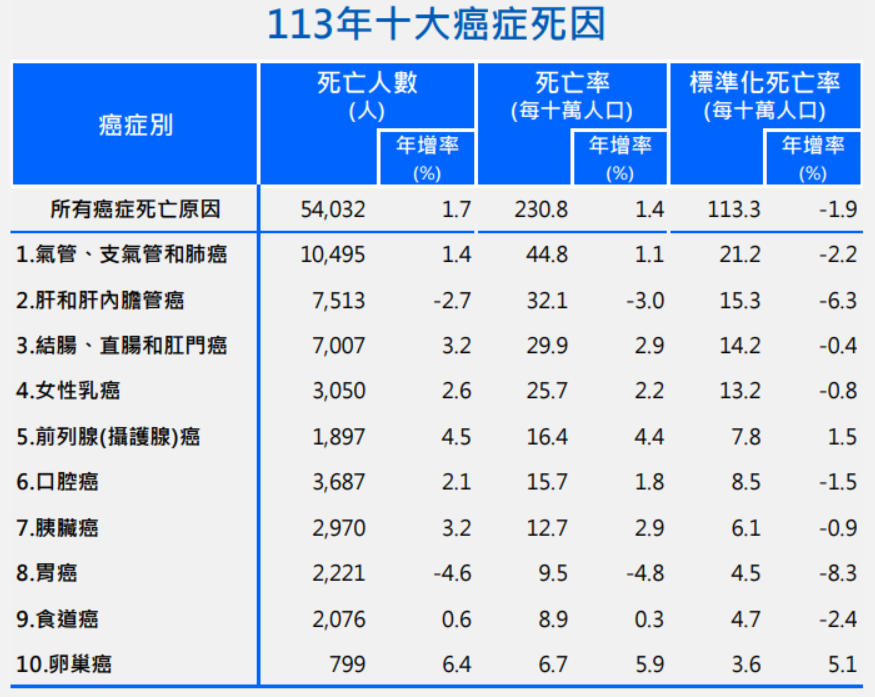
\includegraphics[width=0.6\textwidth]{src/TW_113cancer_stat.png}
            \caption{113 年台灣癌症統計資料}
            \label{fig:113tw_cancer_stat}
        \end{figure}
        \footnotesize
        資料來源:衛福部官網
        
    \end{frame}

    \begin{frame}
        \frametitle{2025 美國癌症統計資料}
        \begin{figure}
            \centering
            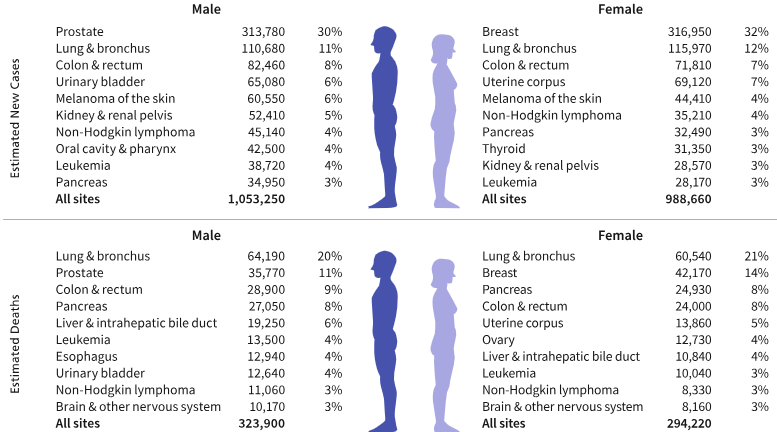
\includegraphics[width=0.8\textwidth]{src/cancer_stat.png}
            \caption{2025 年美國癌症統計資料}
            \label{fig:2025_us_cancer_stat}
        \end{figure}
        \footnotesize
        Siegel, Rebecca L et al. "Cancer Statistics, 2025." CA : a cancer journal for clinicians. 75.1 (2025): 10–45. Web.

    \end{frame}

    % 癌症的分類
    \begin{frame}
        \frametitle{癌症的分類}
        \begin{itemize}
            \item 小細胞肺癌(Small-cell lung carcinoma, SCLC):
                \begin{itemize}
                    \item 佔肺癌的約15 \%。
                    \item 通常與吸煙有關。
                    \item 生長迅速,易於轉移。
                \end{itemize}

            \item 非小細胞肺癌(Non-small-cell lung carcinoma, NSCLC):
                \begin{itemize}
                    \item 佔肺癌的約85 \%。
                    \item 包括腺癌、鱗狀細胞癌和大細胞癌等類型。
                    \item 生長較慢,預後較好。
                \end{itemize}

        \end{itemize}
    \end{frame}

    % 癌症的治療方法
    \begin{frame}
        \frametitle{癌症的治療方法}
        \begin{itemize}
            \item 手術:切除腫瘤組織。
            \item 放射治療:使用高能輻射殺死癌細胞。
            \item 化學治療:使用藥物殺死癌細胞。
            \item 免疫治療:利用免疫系統對抗癌症。
            \item 靶向治療:針對特定分子或基因突變進行治療。
        \end{itemize}
    \end{frame}

    \begin{frame}
        \frametitle{免疫療法的限制}
        免疫治療的原理是隔斷 PD-1 與 PD-L1 的結合,解除免疫抑制,使 T 細胞重新啟動並攻擊腫瘤細胞,因此細胞表面的 PD-L1 會直接影響治療的結果,判斷 PD-L1 表現的準確性對於免疫療法的成功至關重要。小細胞肺癌患者的 PD-L1 表現通常較低,且對免疫治療的反應較差,因此在臨床上,非小細胞肺癌患者的 PD-L1 表現預測更為重要。
        \begin{figure}
            \centering
            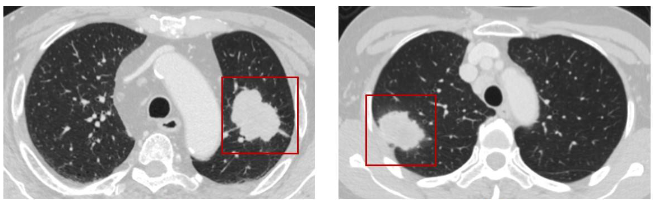
\includegraphics[width=0.6\textwidth]{src/image1.png}
            \caption{左:PD-L1 表現>50\%;右:PD-L1 表現<50\%}
            \label{fig:pd-l1expression}
        \end{figure}
        圖片來源:周姵妤學姐碩士論文
    \end{frame}

    \section{研究目標}
    \begin{frame}
        \sectionpage
    \end{frame}

    % 研究目標
    \begin{frame}
        \frametitle{研究目標}
        \begin{enumerate}
        \item 建立以 MTMAE 為基礎之 PD-L1 表現預測模型
        \item 探討加入對比學習對自監督表徵學習的增強效果。
        \item 在ViT encoder 中嵌入 GNN,建構 patch 間關聯性以提升特徵整合能力。
        \item 評估多模型集成(ensemble)策略對預測穩定性與泛化能力的影響。
        \end{enumerate}
    \end{frame}

    \section{研究方法}
    \begin{frame}
        \sectionpage
    \end{frame}

    \begin{frame}
        \frametitle{研究方法}
        \begin{itemize}
            \item 實驗材料
            \item 模型介紹
            \item 性能指標
        \end{itemize}
    \end{frame}

    % 實驗材料
    \begin{frame}
        \frametitle{實驗材料}
        \begin{itemize}
            \item 資料來源:台大醫院、台大醫院新竹分院、台大醫院雲林分院
            \item 資料類型:非小細胞肺癌患者 CT 與 PD-L1 標記資料
            \item 總樣本數:188 例病患
            \item PD-L1 表現分布:
                \begin{itemize}
                    \item PD-L1 expression ≥ 50\% (+):49 例
                    \item PD-L1 expression < 50\% (−):139 例
                \end{itemize}
        \end{itemize}
    \end{frame}

    \begin{frame}
        \frametitle{GAN 生成的影像}
        為了解決資料稀缺問題,本專案使用實驗室先前所開發之 Gabor-GAN 模型,使用公開資料庫 LIDC-IDRT(Lung Image Database Consortium and Image Database Resource Initiative) 生成 518,064 張2D的樣本以進行預訓練。

    \end{frame}

    % 模型介紹
    \begin{frame}
        \frametitle{模型介紹}
        本專題使用或參考了以下的幾個模型及架構:
        \begin{itemize}
            \item Mask Image Model (MIM)
            \item Masked Autoencoder (MAE)
            \item Vision Transformer (ViT)
            \item Multi-task Masked Autoencoder (MT-MAE)
            \item Simple Contrastive Learning (SimCLR)
            \item Global Contrastive Masked Autoencoder (GCMAE)
            \item Contrastive Masked Autoencoder (CMAE)
        \end{itemize}
    \end{frame}

    % Mask Image Model (MIM)
    \begin{frame}
        \frametitle{Masked Image Model (MIM)}
        \begin{itemize}
            \item 分成 pretrain, finetune
            \item 利用Transfer Learning的概念,將 pretrain 的 encoder 應用於下游任務
            \item pretrain 階段,將輸入影像隨機遮蔽一部分,並預測被遮蔽的部分以學習特徵
        \end{itemize}
    \end{frame}

    % Masked Autoencoder (MAE)
    \begin{frame}
        \frametitle{Masked Autoencoder (MAE)}
        \begin{itemize}
            \item MIM 的一種變體
            \item 利用 Autoencoder 補全被遮蔽的部分以學習特徵
            \item 將 pretrain 的 encoder 應用於下游任務(如:應用於 ViT 模型以進行分類任務)
        \end{itemize}
    \end{frame}

    % MAE architecture
    \begin{frame}
        \begin{figure}
            \centering
            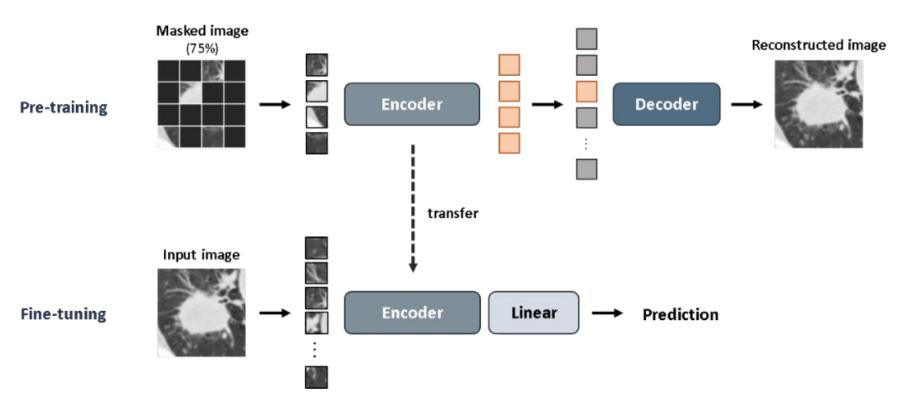
\includegraphics[width=1\textwidth]{src/MAE.png}
            \caption{Masked Autoencoder (MAE) 的架構}
            \label{fig:mae_architecture}
        \end{figure}
        圖片來源:周姵妤學姐的碩士論文
    \end{frame}

    % Vision Transformer (ViT)
    \begin{frame}
        \frametitle{Vision Transformer (ViT)}
        \begin{itemize}
            \item 將影像分割成 patches,並將其視為序列輸入到 Transformer 模型中
            \item 利用自注意力機制學習影像特徵
            \item 使用 CLS token 或是 GAP 處理 token 之後丟到 linear layer 進行分類
        \end{itemize}
    \end{frame}

    % Vision Transformer (ViT) architecture
    \begin{frame}
        \begin{figure}
            \centering
            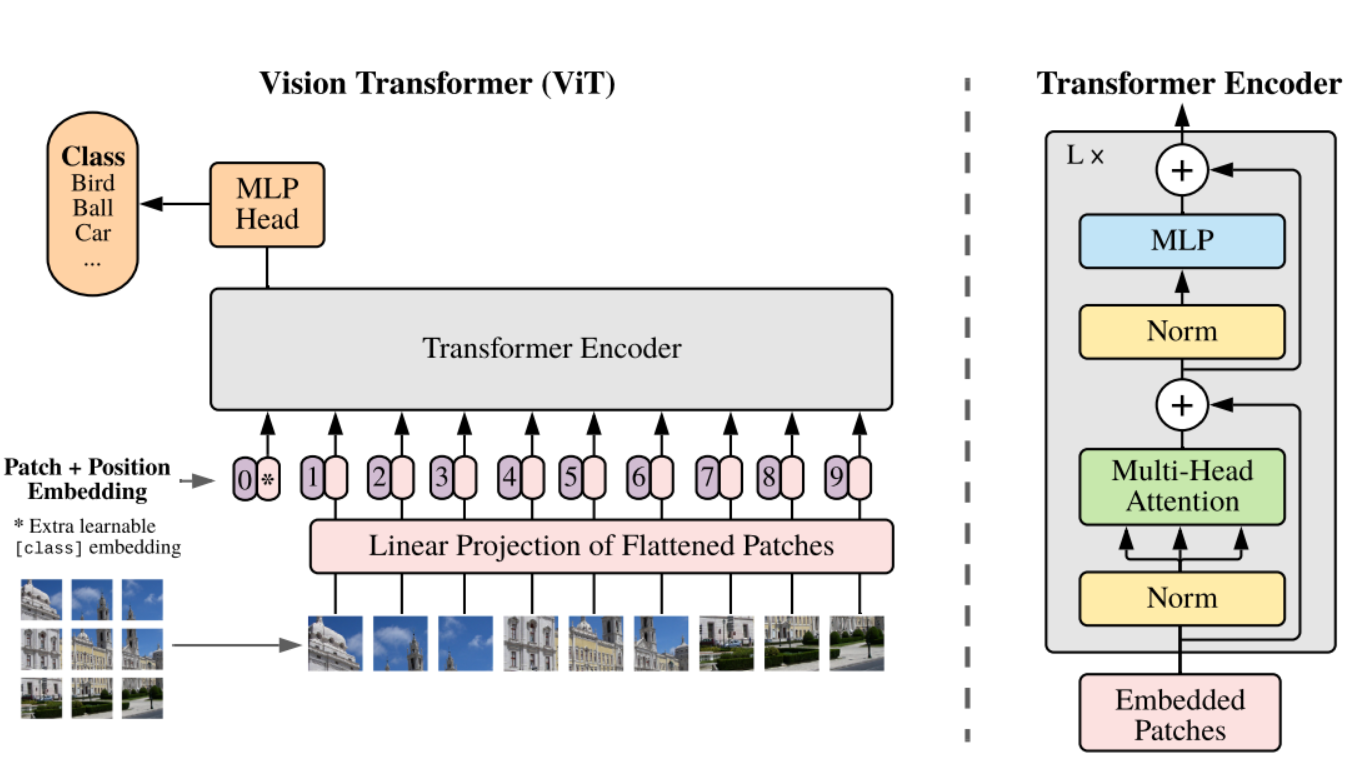
\includegraphics[width=0.8\textwidth]{src/ViT.png}
            \caption{Vision Transformer (ViT) 的架構}
            \label{fig:vit_architecture}
        \end{figure}
        圖片來源:\url{https://arxiv.org/abs/2010.11929}
    \end{frame}

    % Multi-task Masked Autoencoder (MT-MAE)
    \begin{frame}
        \frametitle{Multi-task Masked Autoencoder (MT-MAE)}
        \begin{itemize}
            \item 使用大量 GAN 生成的影像進行 pretrain
            \item 在 pretrain 階段將 MAE 與分割任務結合,使用混合的 Loss 進行優化
            \item 使用訓練好的 encoder 作為下游分割任務的 backbone
        \end{itemize}
    \end{frame}

    % MT-MAE architecture
    \begin{frame}
        \begin{figure}
            \centering
            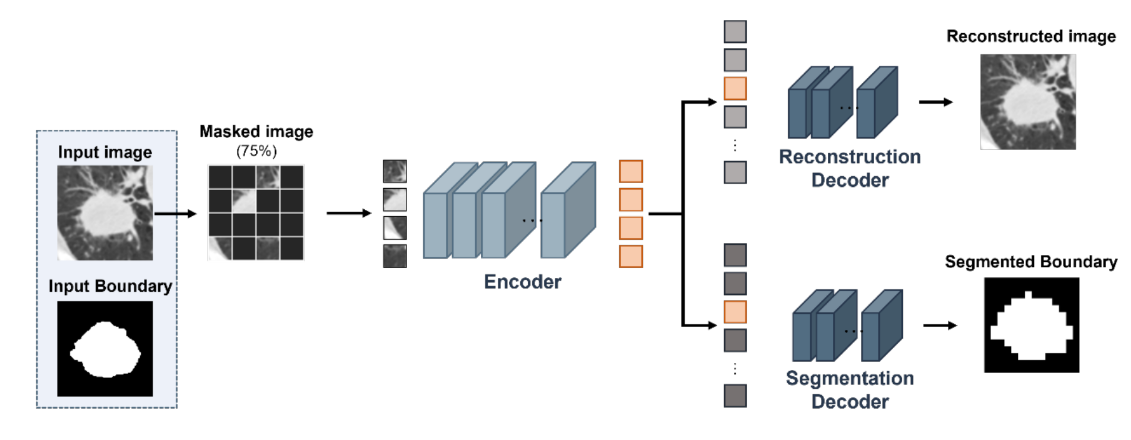
\includegraphics[width=1\textwidth]{src/MTMAE.png}
            \caption{Multi-task Masked Autoencoder (MT-MAE) 的架構}
            \label{fig:mtmae_architecture}
        \end{figure}
        圖片來源:周姵妤學姐的碩士論文
    \end{frame}

    % Simple Contrastive Learning (SimCLR)
    \begin{frame}
        \frametitle{Simple Contrastive Learning (SimCLR)}
        \begin{itemize}
            \item 透過對比學習學習影像特徵
            \item 對同一張影像進行不同的增強,並將其視為正樣本;將不同的影像視為負樣本,使模型學習拉近正樣本,遠離負樣本
            \item 使用 NT-Xent loss 進行優化
        $$
        \ell_{i,j} = -\log \frac{\exp(\mathrm{sim}(\mathbf{z}_i, \mathbf{z}_j)/\tau)}{
            \sum_{k=1}^{2N} \mathbb{1}_{k \neq i}\exp(\mathrm{sim}(\mathbf{z}_i, \mathbf{z}_k)/\tau)}
        $$
        \end{itemize}
    \end{frame}
    % SimCLR architecture
    \begin{frame}
        \begin{figure}
            \centering
            \begin{tikzpicture}
                \node at (0,1.8) (h) {$\longleftarrow\,$Representation$\,\longrightarrow$};
                \node[draw, circle] at (0,-1) (x) {$\,~\mathbf{x}~\,$};
                \node[draw, circle] at (-2.5,0) (x1) {$\tilde{\mathbf{x}}_i$};
                \node[draw, circle] at (2.5,0) (x2) {$\tilde{\mathbf{x}}_j$};
                \node at (-2.5,1.8) (h) {$\mathbf{h}_i$};
                \node at (2.5,1.8) (c) {$\mathbf{h}_j$};
                \node at (-2.5,3) (hh) {$\mathbf{z}_i$};
                \node at (2.5,3) (cc) {$\mathbf{z}_j$};
                \path[->] 
                    (x)  edge [>=latex] node[below,rotate=-25] {$t\sim\mathcal{T}$} (x1)
                    (x)  edge [>=latex] node[below,rotate=25] {$t'\sim \mathcal{T}$} (x2)
                    (x1)  edge [>=latex] node[left,rotate=0] {$f(\cdot)$} (h)
                    (x2)  edge [>=latex] node[right,rotate=0] {$f(\cdot)$} (c)
                    (h)  edge [>=latex] node[left,rotate=0] {$g(\cdot)$} (hh)
                    (c)  edge [>=latex] node[right,rotate=0] {$g(\cdot)$} (cc);
                \path[<->]
                    (hh)  edge [>=latex] node[above,rotate=0] {Maximize agreement} (cc);
            \end{tikzpicture}
            \caption{SimCLR 架構圖}
        \end{figure}
    \end{frame}

    % Global Contrastive Masked Autoencoder (GCMAE)
    \begin{frame}
        \frametitle{Global Contrastive Masked Autoencoder (GCMAE)}
        \begin{itemize}
            \item 結合 MAE 與 SimCLR 的思想
            \item 利用 MAE 學習局部特徵;結合 GCLR 學習全局特徵
        \end{itemize}
    \end{frame}

    % GCMAE architecture
    \begin{frame}
        \begin{figure}
            \centering
            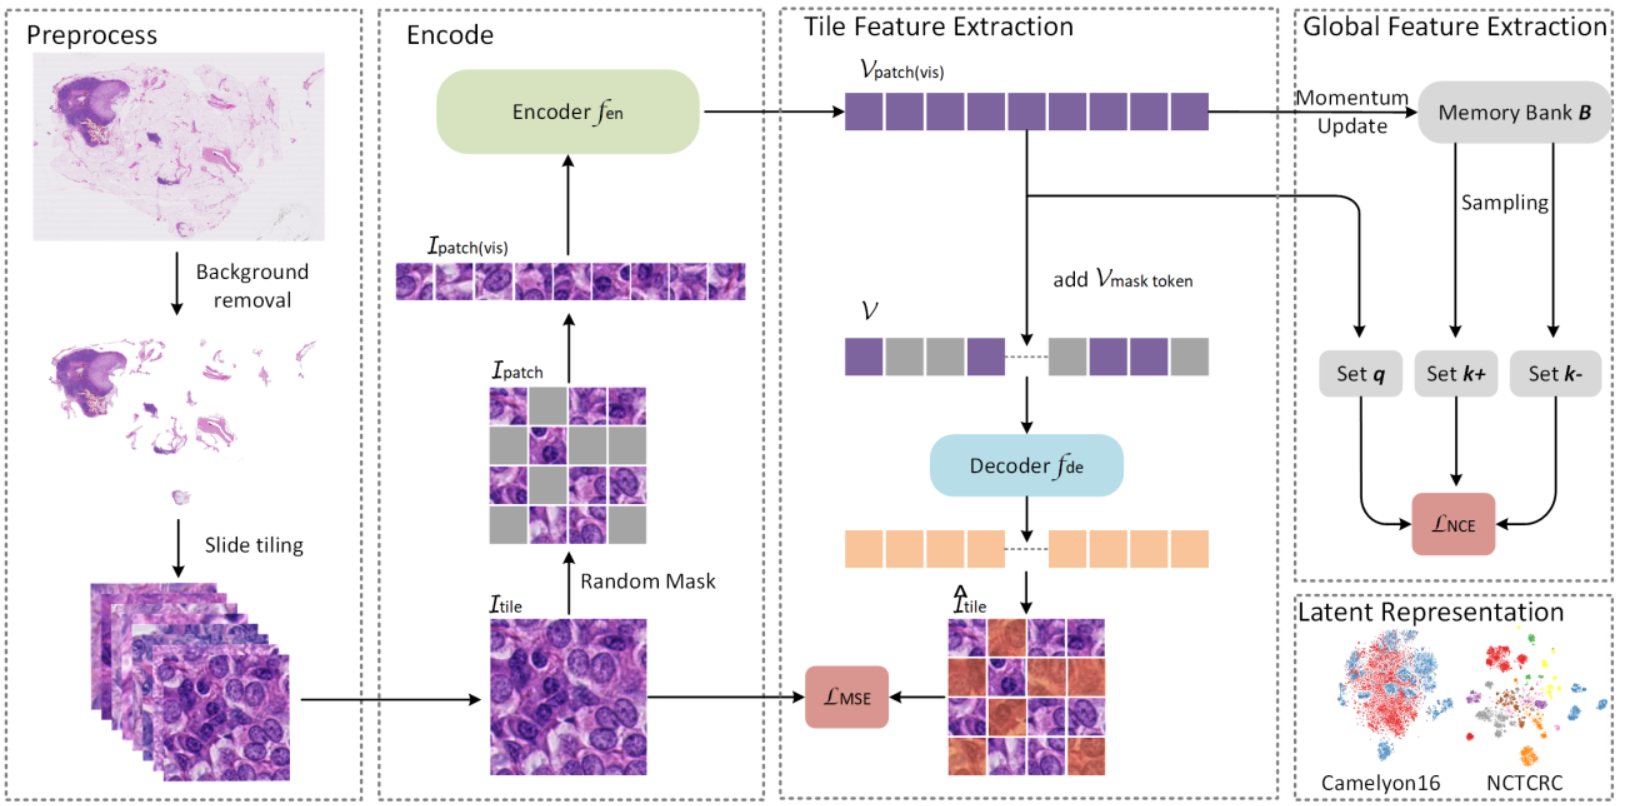
\includegraphics[width=1\textwidth]{src/GCMAE.png}
            \caption{Global Contrastive Masked Autoencoder (GCMAE) 的架構}
            \label{fig:gcmae_architecture}
        \end{figure}
        圖片來源:\url{https://arxiv.org/abs/2205.09048}
    \end{frame}

    % Contrastive Masked Autoencoder (CMAE)
    \begin{frame}
        \frametitle{Contrastive Masked Autoencoder (CMAE)}
        \begin{itemize}
            \item 一樣結合 MAE 與對比學習
            \item 利用孿生網路結構,結合 MAE 與 CL
        \end{itemize}
    \end{frame}

    % CMAE architecture
    \begin{frame}
        \begin{figure}
            \centering
            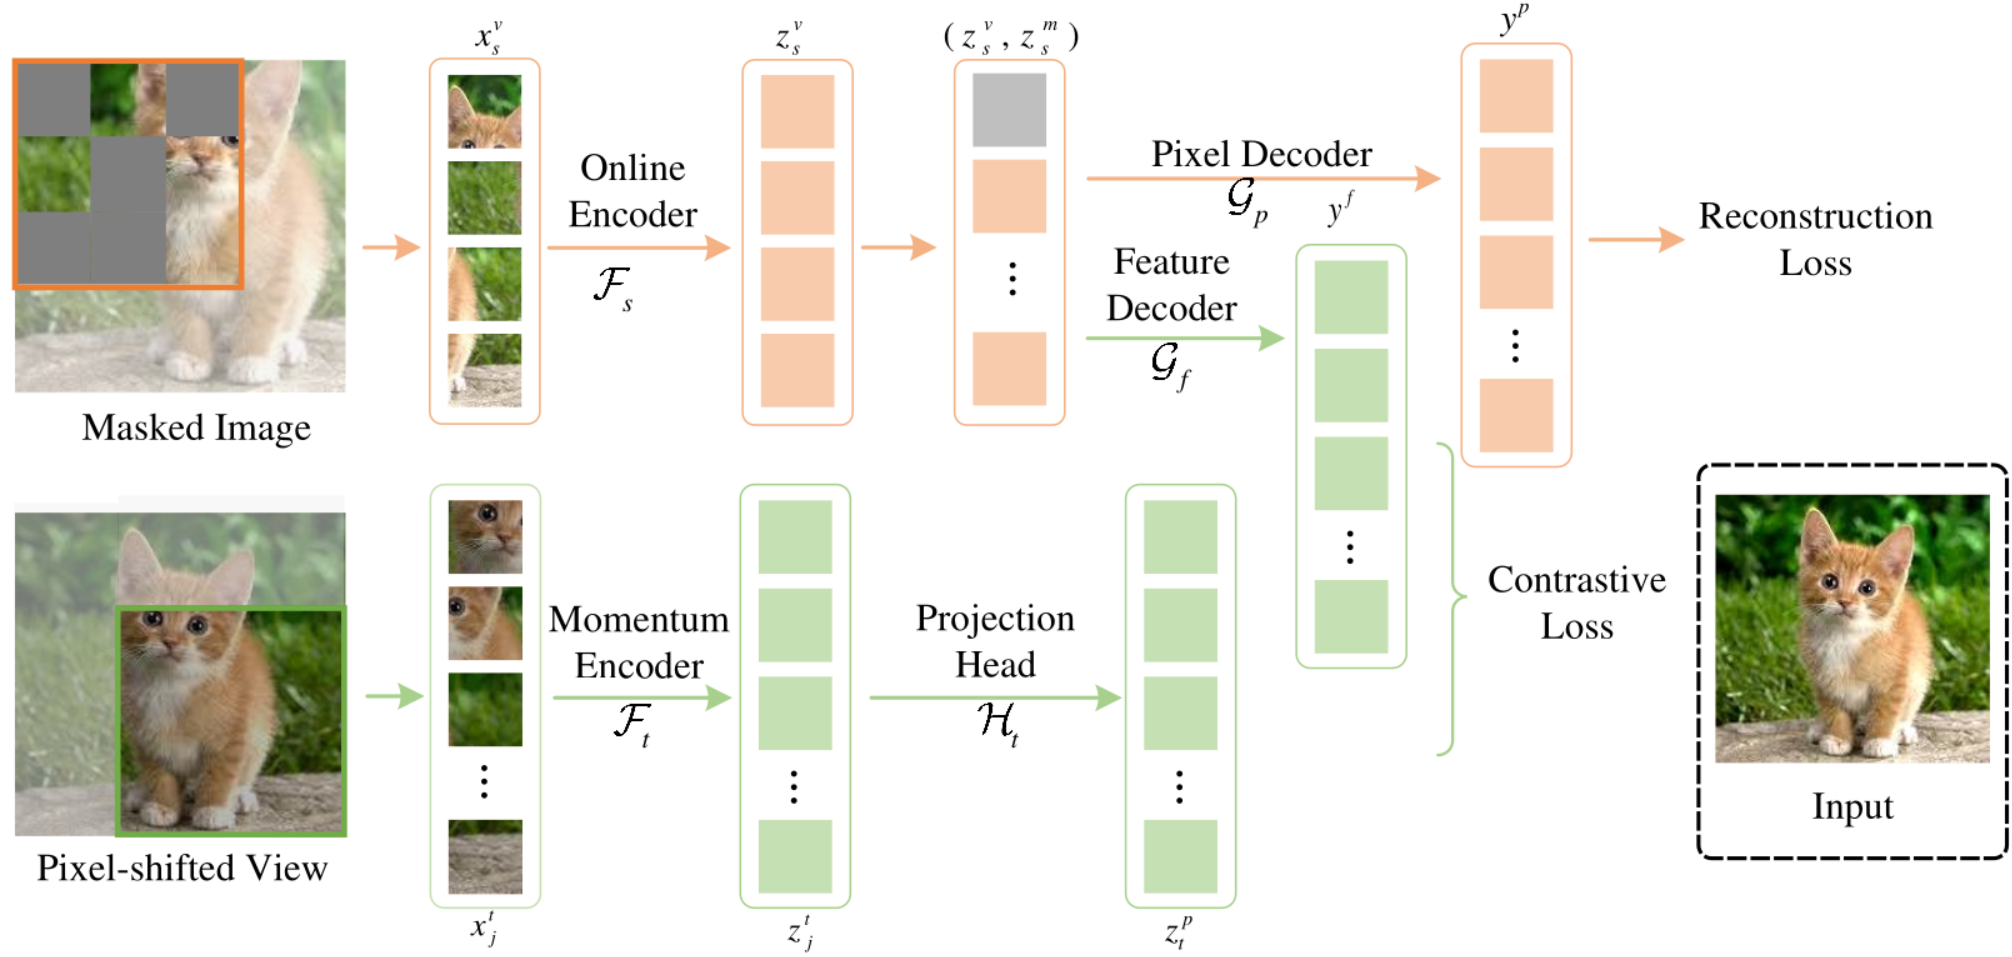
\includegraphics[width=1\textwidth]{src/CMAE.png}
            \caption{Contrastive Masked Autoencoder (CMAE) 的架構}
            \label{fig:cmae_architecture}
        \end{figure}
        圖片來源:\url{https://arxiv.org/abs/2207.13532}
    \end{frame}

    % 性能指標
    \begin{frame}
        \frametitle{性能指標}
        \begin{itemize}
            \item 正確率(Accuracy):預測正確的樣本數與總樣本數之比。
            \item 靈敏度(Sensitivity):預測為正樣本的實際正樣本數與總實際正樣本數之比。
            \item 特異度(Specificity):預測為負樣本的實際負樣本數與總實際負樣本數之比。
            \item AUC(Area Under the Curve):ROC 曲線下的面積,用於評估模型在不同閾值下的分類性能。
        \end{itemize}
    \end{frame}

    % AUC
    \begin{frame}
        \begin{figure}
            \centering
            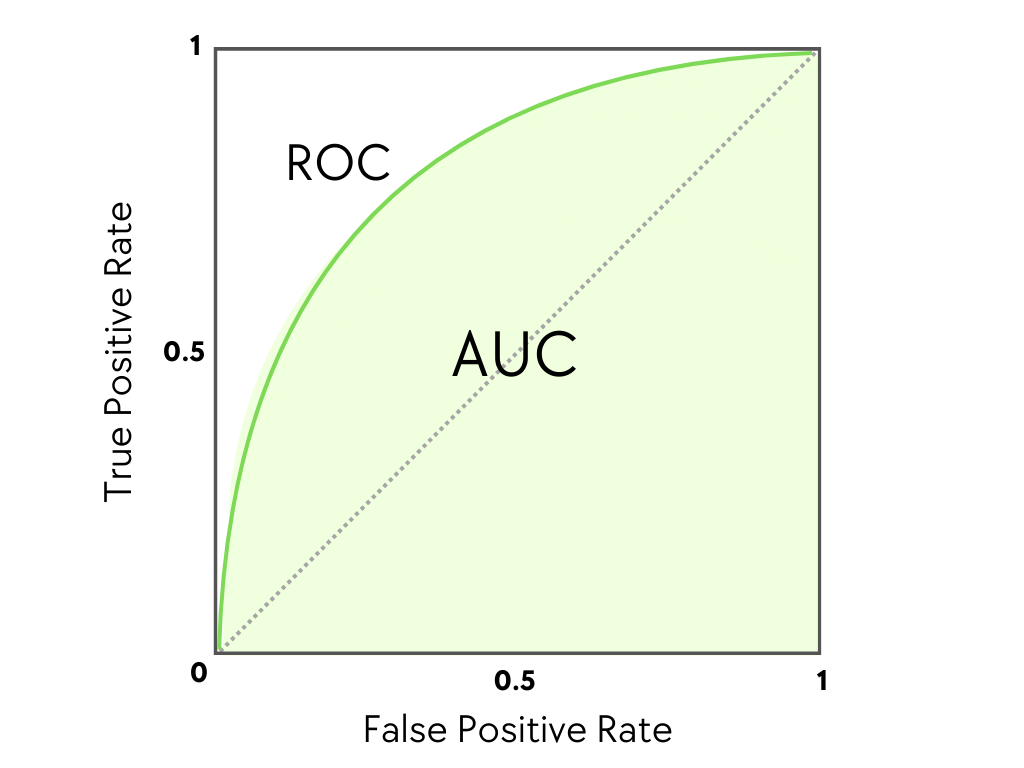
\includegraphics[width=0.6\textwidth]{src/auc.png}
            \caption{ROC 曲線及其 AUC 值}
            \label{fig:roc_curve_example}
        \end{figure}
        圖片來源:https://www.blog.trainindata.com/auc-roc-analysis/
    \end{frame}

    \section{研究結果與討論}
    \begin{frame}
        \sectionpage
    \end{frame}

    % 重現
    \begin{frame}
        \frametitle{對照組-還原論文的結果}
        \begin{itemize}
            \item 參考周姵妤學姐的碩士論文,重現 MTMAE 模型的架構與訓練流程:
            \begin{enumerate}
                \item 利用 PyTorch 框架實現模型,並使用學姐留下來的 CT 影像與 PD-L1 標記資料進行訓練
                \item 進行 200 個 epoch 的預訓練之後得到 MTMAE 模型的權重
                \item 使用真實的醫學影像進行微調,並評估模型在 PD-L1 表現預測任務上的準確率
            \end{enumerate}

            \item 最終多次實驗得到的 AUC 平均值為 0.6168
            \item 結果與學姐論文中所報告相差甚遠,推測是因為資料量太少,不同的排列順序會導致模型預測結果有很大差異
        \end{itemize}
    \end{frame}

    % 微調的方法
    \begin{frame}
        \frametitle{微調的方法}
        \begin{figure}
            \centering
            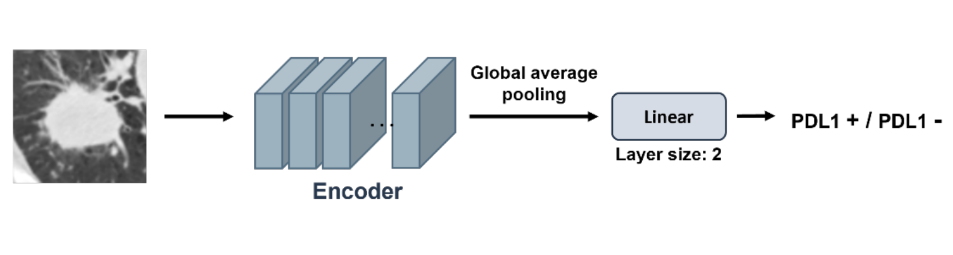
\includegraphics[width=0.8\textwidth]{src/finetune.png}
            \caption{微調階段的架構}
            \label{fig:finetune_architecture}
        \end{figure}
    \end{frame}

    % SimCLR 的訓練
    \begin{frame}
        \frametitle{SimCLR 的訓練}
        \begin{figure}
            \centering
            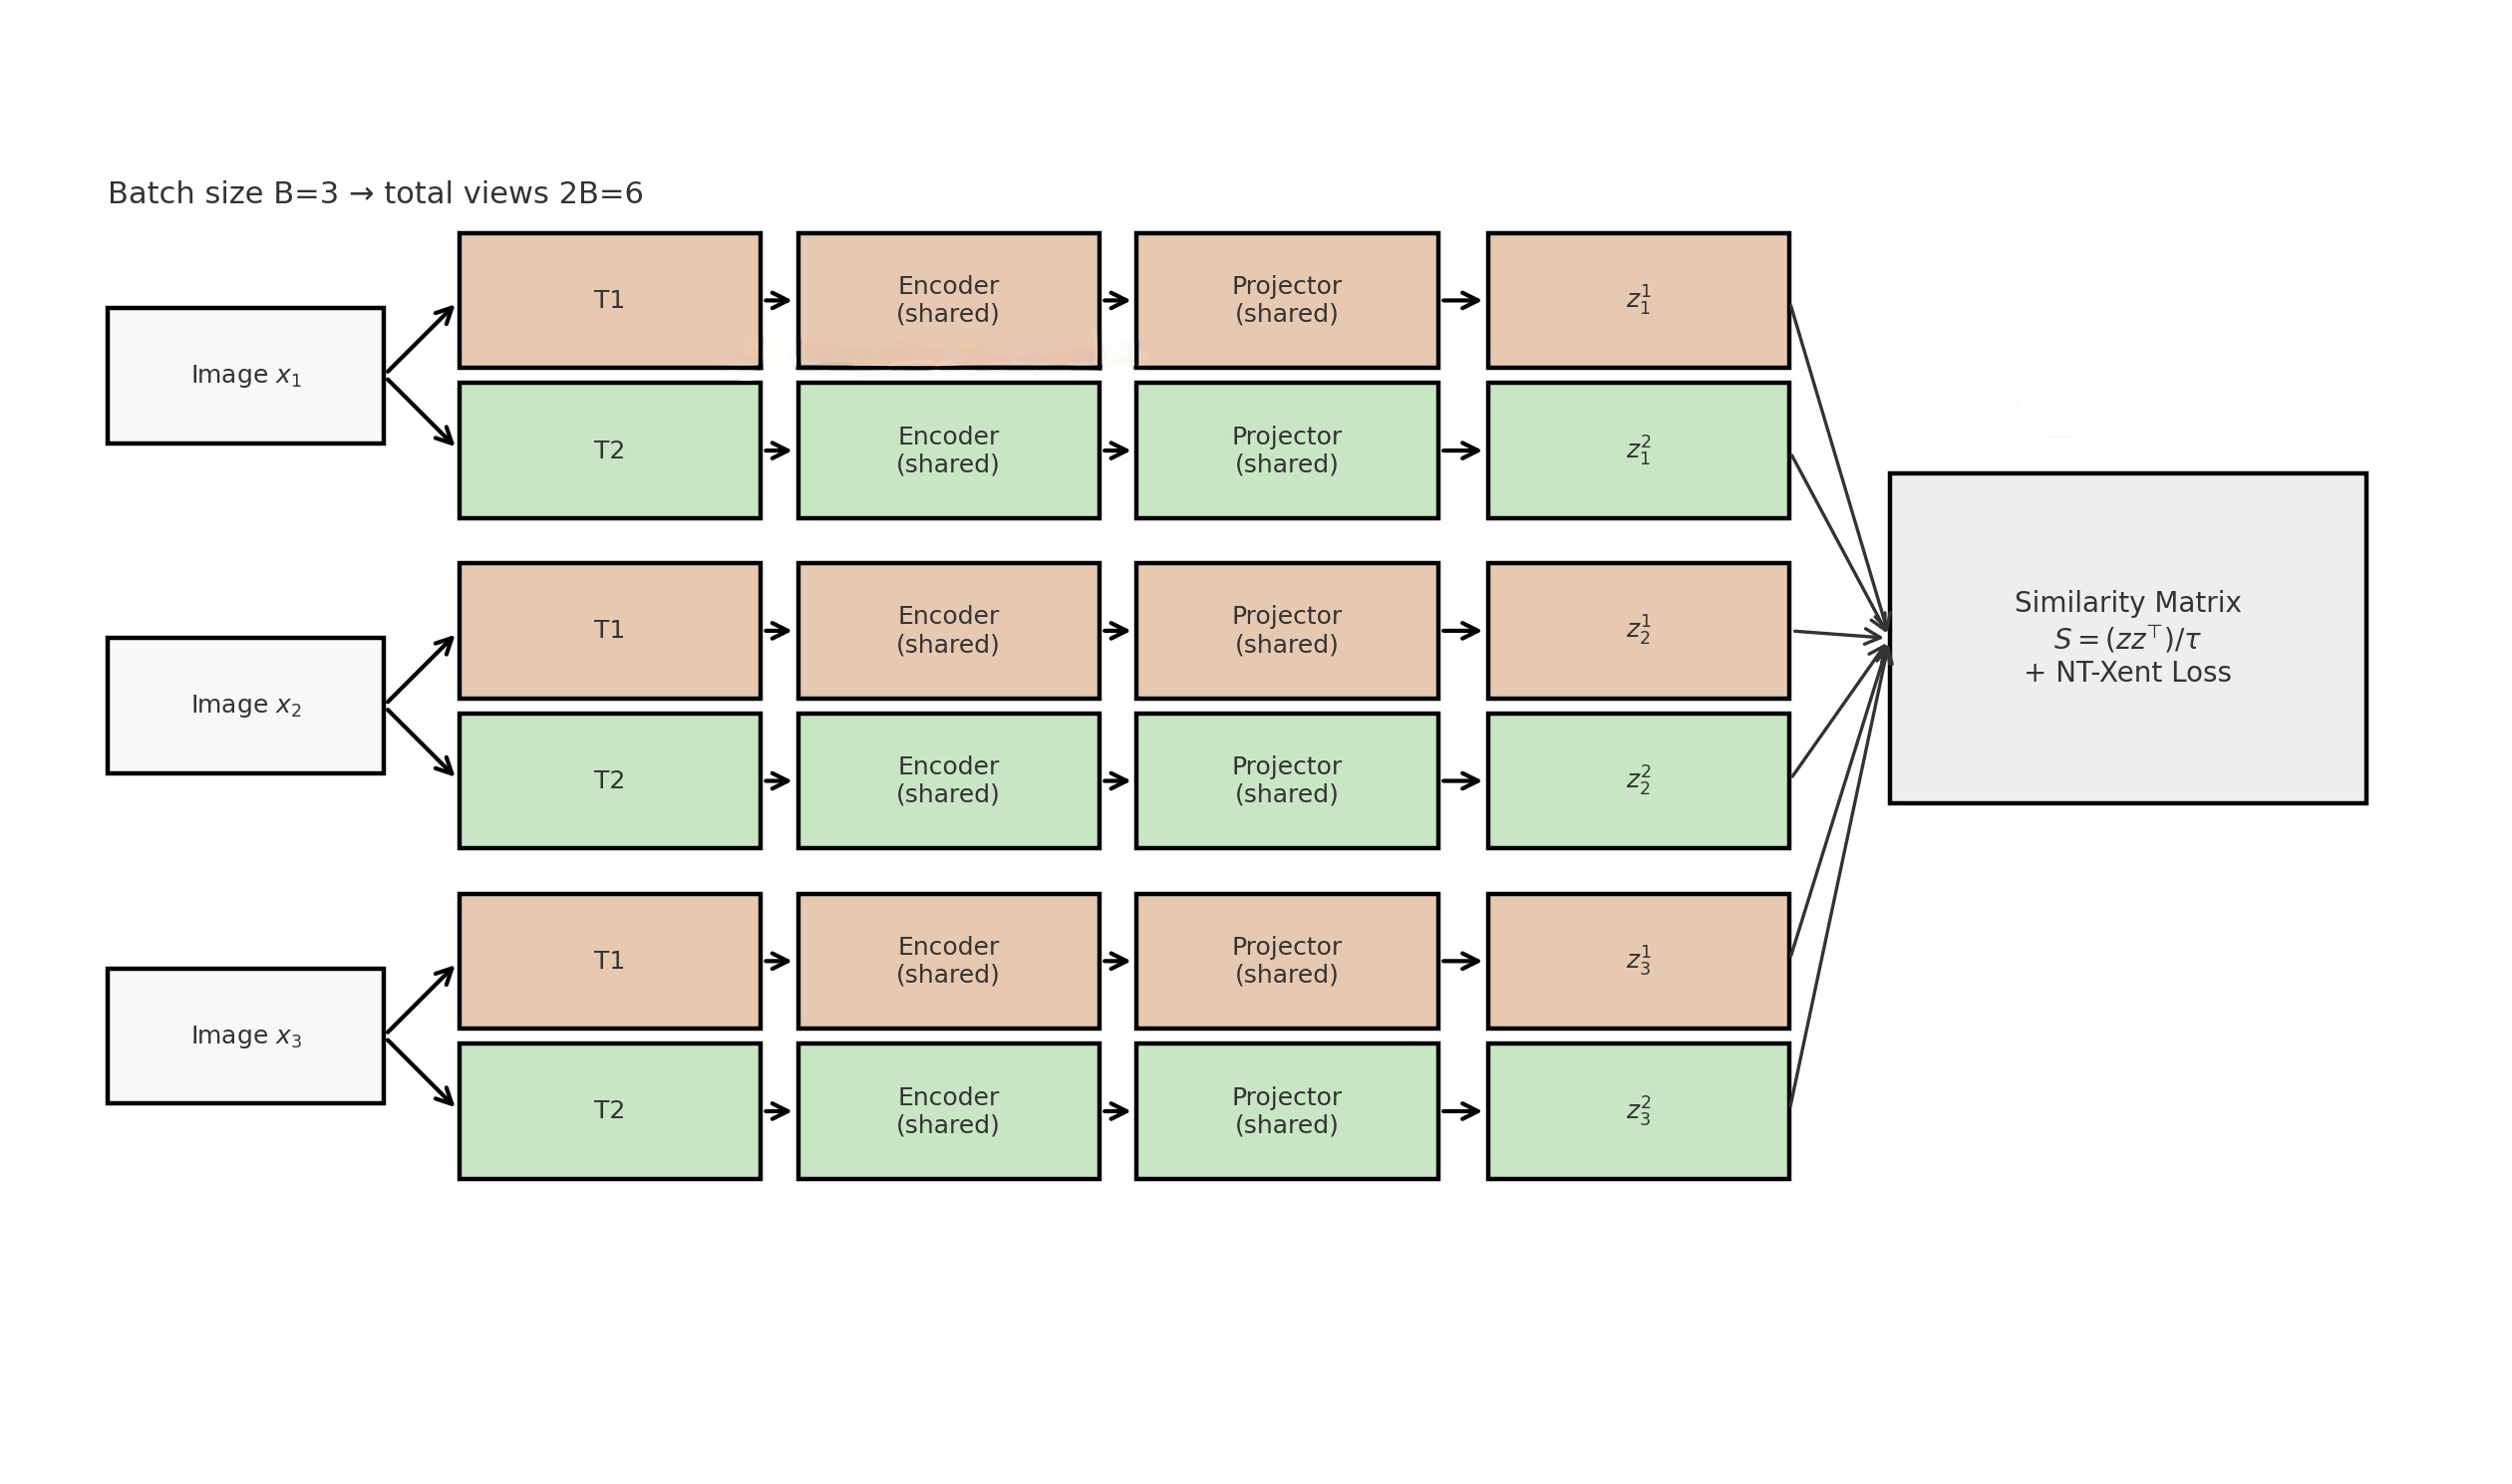
\includegraphics[width=0.9\textwidth]{src/SimCLR_framework.jpg}
            \caption{SimCLR 的訓練方式}
            \label{fig:simclr_training_process}
        \end{figure}
    \end{frame}

    % SimCLR 的訓練結果
    \begin{frame}
        \frametitle{SimCLR 的訓練結果}
        \begin{table}[h]
        \centering
        \begin{tabular}{lcc}
        \toprule
        & \textbf{純粹使用simCLR} & \textbf{MTMAE + SimCLR 微調} \\
        \midrule
        AUC          & 0.4395 & 0.5000 \\
        ACC          & 0.4839 & 0.4355 \\
        \bottomrule
        \end{tabular}
        \caption{SimCLR 方法實驗結果比較}
        \label{tab:simclr-results}
        \end{table}
        由結果可知,純粹使用 SimCLR 訓練的模型表現較差,可能是破壞了原有的特徵學習結構。查閱資料後,我找到了 CMAE 的方法,這個方法結合了 MAE 與 SimCLR 的優點,能夠更好地學習影像特徵。
    \end{frame}

    % CMAE 的訓練
    \begin{frame}
        \frametitle{CMAE 的訓練}
        由於完整使用 CMAE 預訓練的時間太長,因此我使用了 CMAE 的預訓練權重,和 MAE 的權重進行對比。這兩個權重都是在 ImageNet 上預訓練的。
        \begin{table}[h]
        \centering
        \begin{tabular}{lcc}
        \toprule
        & \textbf{CMAE} & \textbf{MAE} \\
        \midrule
        AUC          & 0.5625 & 0.5584 \\
        ACC          & 0.7419 & 0.6452 \\
        \bottomrule
        \end{tabular}
        \caption{CMAE 方法實驗結果比較}
        \label{tab:CMAE-results}
        \end{table}       
        雖然效果不彰,但仍可看出 CMAE 在某些指標上優於 MAE,或許代表了 CMAE 的潛力。
    \end{frame}

    \begin{frame}
        \frametitle{類似模型集成的方法}
        \begin{table}[h]
        \centering
        \begin{tabular}{lccc}
        \toprule
        & \textbf{5-fold(輪流遮住資料)} & \textbf{5-fold(訓練資料固定} & \textbf{150 個 epoch} \\
        \midrule
        AUC          & 0.6984 & 0.5645 & 0.6644\\
        ACC         & 00.7419 & 0.5421 & 0.7419\\
        \bottomrule
        \end{tabular}
        \caption{5-fold 方法實驗結果比較}
        \label{tab:5-fold-results}
        \end{table}       
    \end{frame}


    \section{結論與展望}
    \begin{frame}
        \sectionpage
    \end{frame}
    \begin{frame}
        \frametitle{結論與展望}
        \begin{itemize}
            \item 結合 SimCLR 與 MAE 的方式有些問題,或許可以參考 CMAE 或是 GCMAE 的方法。
            \item CMAE 的方法有一定的潛力
            \item 未來預計嘗試:
            \begin{enumerate}
                \item 使用完整的 CMAE 模型進行預訓練
                \item 使用孿生網路的概念結合 MT-MAE 與 CMAE
                \item 讓模型不再僅判斷正負,而是將 PD-L1 的表現分成不同層級
                \item 嘗試將正確的 k-fold 模型集成策略應用於微調階段,將多個不同的模型進行集成
            \end{enumerate}
        \end{itemize}
    \end{frame}

    \begin{frame}
        \frametitle{參考資料}
            \begin{enumerate}
                \footnotesize
                \item 周姵妤,肺部電腦斷層掃描之非小細胞癌 PD-L1 表現預測 :結合遮蓋圖像模型與生成對抗網路,碩士論文,國立臺灣大學,2024。
                \item Devlin, Jacob, et al. "Bert: Pre-training of deep bidirectional transformers for language understanding." Proceedings of the 2019 conference of the North American chapter of the association for computational linguistics: human language technologies, volume 1 (long and short papers). 2019.
                \item Bao, Hangbo, et al. "Beit: Bert pre-training of image transformers." arXiv preprint arXiv:2106.08254 (2021).
                \item He, Kaiming, et al. "Masked autoencoders are scalable vision learners." Proceedings of the IEEE/CVF conference on computer vision and pattern recognition. 2022.
                \item Chen, Ting, et al. "A simple framework for contrastive learning of visual representations." International conference on machine learning. PmLR, 2020.
                \item Quan, Hao, et al. "Global contrast-masked autoencoders are powerful pathological representation learners." Pattern Recognition 156 (2024): 110745.
                \item Huang, Zhicheng, et al. "Contrastive masked autoencoders are stronger vision learners." IEEE Transactions on Pattern Analysis and Machine Intelligence 46.4 (2023): 2506-2517.
            \end{enumerate}
    \end{frame}
\end{document}